\begin{figure}
    \centering
    \begin{tikzpicture}
        \def\layerthick{1.5}; \def\sidelen{5}; \def\fluidlen{1.5}; \def\arrowspacing{0.4}

        % Diagram
        \node at (-.5, 3.5) {a)};
        % Fill geometries 
        \fill[porous] (0, 0) rectangle ++ (\sidelen, \layerthick);
        \shade[left color=white, right color=porous] (0, 0) rectangle ++ (.4, \layerthick);
        \shade[right color=white, left color=porous] (\sidelen-.4, 0) rectangle ++ (.4, \layerthick);
        \shade[top color=white, bottom color=blue!30!white] 
        (0, \layerthick) rectangle ++ (\sidelen,\fluidlen);
        \shade[bottom color=white, top color= blue!30!white] 
        (0, 0) rectangle ++ (\sidelen, -\fluidlen);
        
        % Lines and arrows
        \draw[dashed] (0, 0) -- (\sidelen, 0);
        \draw[dashed] (0, \layerthick) -- (\sidelen, \layerthick);
        \draw[-Latex] (0, 0) -- (0.7, 0) node[near end, above right] {$x_1$};
        \draw[-Latex] (0, 0) -- (0, 0.7) node[near end, above right] {$x_2$};
        \draw[-Latex] (2, \layerthick/3) -- (3.5, \layerthick/3) node[midway, above] {$ k_1$};
        \draw[Latex-Latex] (-\arrowspacing, 0) -- (-\arrowspacing, \layerthick) node[midway, left] {$H$};

        % Radiated amplitudes 
        \draw[-Latex,thick,decorate,decoration={snake,amplitude=5pt,pre length=0pt,post length=6pt}] 
        (1, \layerthick + \arrowspacing) -- ++(1,0.5) node[very near end, above left] {$ k_2^{(f+)}$};
        \draw[-Latex,thick,decorate,decoration={snake,amplitude=5pt,pre length=0pt,post length=6pt}] 
            (2, -\arrowspacing) -- ++(1,-0.5) node[very near end, below left ] {$ k_2^{(f-)}$};
        
        % Right geometry legends 
        \draw[Circle-] (\sidelen-\arrowspacing, \layerthick/2) -- (\sidelen+.7, \layerthick/2) node[right] {$\Omega_1$};
        \draw[Circle-] (\sidelen-\arrowspacing, \layerthick) -- (\sidelen+.7, \layerthick) node[right] {$\Gamma_1$};
        \draw[Circle-] (\sidelen-\arrowspacing, 0) -- (\sidelen+.7, 0) node[right] {$\Gamma_0$};

        \node at (7, 3.5) {b)};
        \node[below right] at (7.5, 3.5) {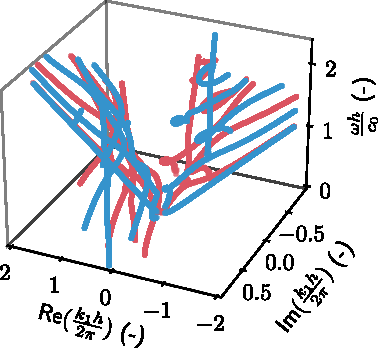
\includegraphics{figures/symmetry_modes2.pdf}};

        \node at (-0.5, -3) {c)};
        \node[below right] at (-1, -3.2) {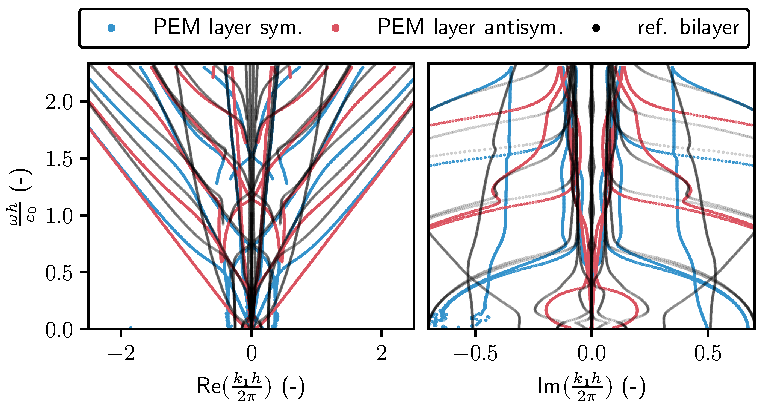
\includegraphics{figures/disp_pem_plate.pdf}};
    \end{tikzpicture}
    \caption{a) Sketch of the single layer poroelastic structure geometry. b) 3D view of the complex wavenumber-real frequency dispersion relation and c) real and imaginary parts of the dispersion relation. The branches of the symmetric and antisymmetric modes are represented by blue and red curves respectively. The dispersion relation of the two-layer elatsic-poroelastic system studied in Section \ref{Section3} are reminded with black lines.}
    \label{fig:fluid_coupled_poroelastic}
\end{figure}
        
